% This is samplepaper.tex, a sample chapter demonstrating the
% LLNCS macro package for Springer Computer Science proceedings;
% Version 2.20 of 2017/10/04
%
\documentclass[runningheads]{llncs}
%
\usepackage{graphicx}
\usepackage{hyperref}
\usepackage{float}

\begin{document}
%
\title{Smart lecture rooms at universities}

\author{Group ID 07: Yunxuan Li \and
Zhixian Li \and
Jingxi Zhang}

\institute{Service Computing Department, IAAS, University of Stuttgart
\email{st119871,st146584,st141130@stud.uni-stuttgart.de}}
%
\maketitle              % typeset the header of the contribution
%
\begin{abstract}
This project is part of the lecture smart cities and internet of things \cite{ref_url1}. A lecture room is the most often and common place that student will go in an university. However, it is not easy to keep everyone in a lecture room comfortable, health and productive while have the lecture room itself secure and energy efficient. To achieve this goal, we plan to develop a smart lecture room system that uses different sensors to monitor the current state of a lecture room and automatically make decisions based on the information it has gathered.

\keywords{Lecture room  \and Smart building \and Comfortable \and Energy efficiency.}
\end{abstract}
%
%
%
\section{System Introduction}
For students, a lecture room might be the most often place we stay in an university. However, it’s hard to have everyone comfortable in a lecture room, for example, someone might want to have fresh air, but it could be too cold for others. In addition, it would be hard to keep everyone productive, for example, there might be a reflection on black board, but the professor did not notice.  Furthermore, it could also be hard to keep the security and energy efficiency of a lecture room, for example, the door of a lecture could be left open and the light of a lecture room could be left on after a lecture is done. Therefore, we want to develop a smart lecture room system that not only tries to make everyone in the room comfortable and productive but also keeps the lecture room secure and energy efficient. \\
To accomplish this goal, we decided to use different sensors in a lecture room that monitor the temperature, the weather, the air quality and so on. Based on these sensors, we will develop an automate system that decides when to make actions such like open the window or close the light. Unfortunately, the system cannot carry out all these actions automatically due to limited hardware support. Thus, the decision will be sent to the professor or the room management so that they can do the corresponding actions.


\section{System Analysis}
We will describe the system functionality using user stories in the following, where these user stories will be the main focus of our project.
\begin{itemize}
\item As a lecturer I want the room to automatically adjust light and curtains, so that my powerpoint is clearly visible.\\

\item As a student or a lecturer I want the room temperature and humidity to be as ideal as possible for a lecture.\\

\item As a manager of the cost of the buildings I want the system to idealize the energy so that the cost is minimized.\\
\end{itemize}

The following user stories will be additional features. Condition for implementing these will be the time we can invest into the project and the cost of the hardware.\\ 
These two user stories involve a door lock. As a physical door lock with electric mechanism is expensive we will stick to a simplification like sending an email or using a light to indicate the state of the door.
\begin{itemize}
\item As a caretaker of the building I want the doors to be locked after lecture hours to be able to guarantee the security of the building. \\

\item As a student I want the doors to be open before lecture to be able to prepare my utils for the lecture.\\
\end{itemize}

\section{System Architecture Design}
The user interface is realized on a laptop which communicates with a raspberry Pi where our system runs. The learning algorithm is also on the raspberry Pi. In the user interface light and air condition can also be manually adjusted.\\
With weather forecast, temperature sensors and CO2 sensors we adjust the air conditioner and the windows. \\
An infrared camera is connected as a sensor to recognize people in the room. As there might be students discussing with a lecturer after the lecture, the room must not lock the doors. \\
Our Ubiquitous Layer wil process the data received from our sensors and combine it with calendar and weatherforecast data. Our planner service is the part where our ai planning come into play. It makes a decision based on the data given. The decision is forewarded to the actuators to carry out an action.\\

Figure \ref{fig:SystemArchitecture} shows our system Architecture.\\

\begin{figure}[H]
\centering
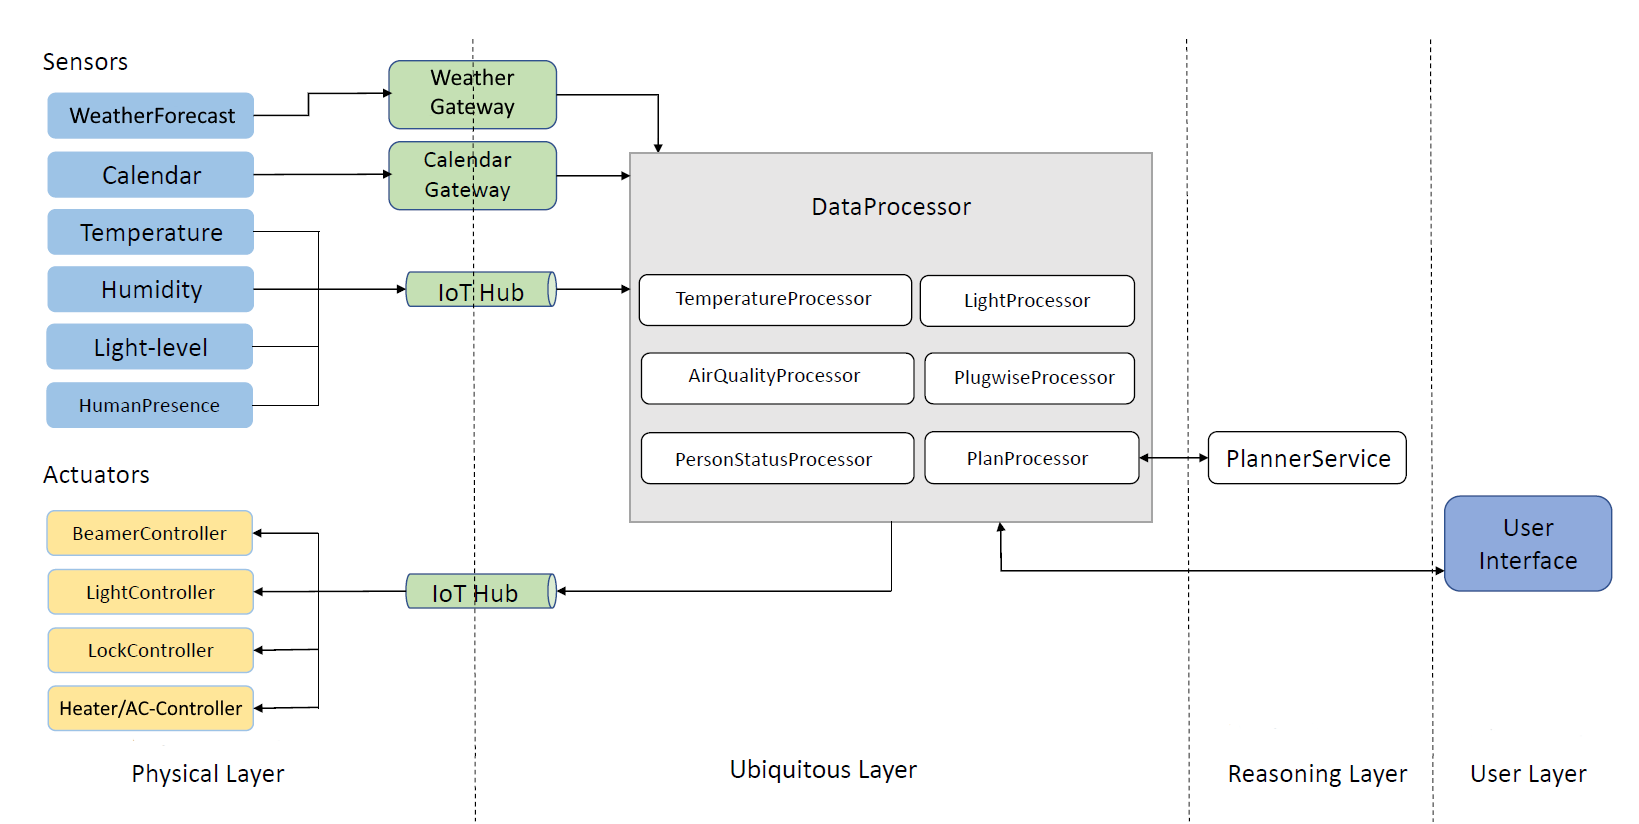
\includegraphics[width=1.0\textwidth]{../img/IotDiagram.png}
\caption{SystemArchitecture}
\label{fig:SystemArchitecture}
\end{figure}




%Components:


%Presentation layer\\
%Application logic layer\\
%Data layer \\

%
% ---- Bibliography ----
%
\bibliographystyle{splncs04}
\bibliography{mybib}

All links were last followed on \today

\end{document}
